
\section{Ejercicio 2: Problemas en el camino}
    % 1. Describir detalladamente el problema a resolver dando ejemplos del mismo y sus soluciones.
	\subsection{Descripción del problema}

	\begin{figure}[ht]
		\begin{center}
			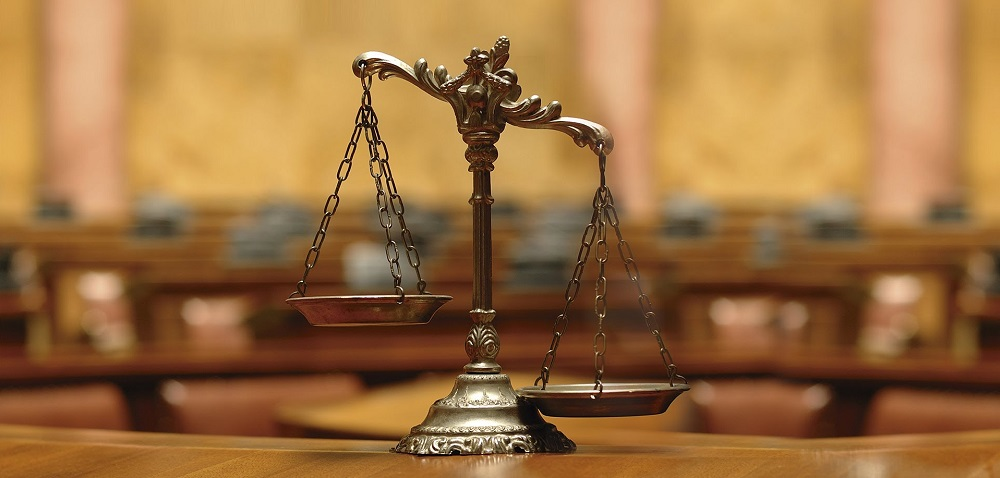
\includegraphics[width=0.5\columnwidth]{imagenes/balanza.jpg}
			\caption{Equilibro}
		\end{center}
	\end{figure}

	Luego de cruzar el puente, el equipo se encuentra en una habitación amplia con una puerta, la cual está cerrada. En el medio de la habitación hay una balanza de dos platillos, la cual contiene sobre su platillo izquierdo una llave que abre la puerta de la habitación. Al retirar la llave, se cambia el equilibro de la balanza, lo cual hace que se cierre la entrada de la habitación. La llave no sirve para abrir la puerta y lo único que puede realizar el equipo es recompener el equilibro de la balanza utilizando un conjunto de pesas de potencia de 3 distintas. Es decir, sólo disponen de una sóla pesa de cada potencia de 3. Los datos de entrada y de salida para el problema son los siguientes: 

	~

	\textbf{Formato de entrada:} El único dato de entrada es un entero $P$ que representa el peso de la llave.

	\begin{tabular}{ll}
		\texttt{P}
	\end{tabular}

	~

	\textbf{Salida:} La salida consiste en dos enteros $S$ y $T$ que representan la cantidad de pesas que hay que colocar en el platillo izquierdo y el derecho respectivamente, seguidas de otra línea con los valores de las pesas que se deben colocar del platillo izquierdo ordenadas de menor a mayor y finalmente otra línea con los valores de las pesas del platillo derecho, también con el mismo orden.

	\begin{tabular}{ll}
		\texttt{S} & \texttt{T} \\
		\texttt{I1 ...} & \texttt{...IS} \\
		\texttt{D1 ...} & \texttt{...DT} \\
	\end{tabular}

	~

	Se tiene como restricción que el peso $P$ está en el siguiente rango: 1$<=$ $P$ $<=$ $10^{15}$. La complejidad temporal debe ser a lo sumo $\ord(\sqrt{P})$. 

    % 2. Explicar de forma clara, sencilla, estructurada y concisa, las ideas desarrolladas para la resolución del problema. Utilizar pseudocódigo y lenguaje coloquial (no código fuente). Justificar por qué el procedimiento resuelve efectivamente el problema.
    \subsection{Solución propuesta}

	La idea propuesta para la resolución del problema consiste en buscar cómo obtener una representación del número $p$. Si se consigue una representación del mismo se puede equilibrar la balanza. Primero nos abtraemos de las restricciones del problema y pensamos que cualquier número $a$ $\in$ \mathds{N} admite un desarrollo en base $d$, utilizando sólo símbolos comprendidos en el rango de 0 a $d-1$. Como se dispone de sólo pesas que son potencias de 3, se decide utilizar la base 3 para representar el número. Si el problema no tuviera la restricción de que sólo se dispone de una pesa de cada potencia de 3, la resolución sería trivial ya que sólo consiste en obtener el desarrollo en base 3 del número $p$ (que es un dato de entrada y que se asume que su desarrollo es en base 10) y poner tantas pesas de cada potencia de 3 (hasta 2 por potencia ya que en base 3, sólo se pueden utilizar los símbolos 0, 1 y 2) como indique el desarrollo, en el plato de la izquierda de la balanza para obtener el mismo peso $p$. Pero la restricción de que sólo se dispone de una sóla pesa de cada potencia de 3 hace que dicha solución no funcione. No obstante, teniendo en cuenta que en la balanza, las pesas que se colocan en el lado derecho 'restan' el peso colocado en el plato izquierdo se puede pensar en una solución en la cual cuando se tengan que utilizar dos pesas de la misma potencia, se puedan reemplazar por el uso de una pesa mayor colocada en el plato izquierdo (la cual se interpretaría como suma de dicha potencia de 3) y el uso de otra pesa colocada en el plato derecho (la cual se interpretaría como resta de dicha potencia de 3). Para lograr que la suma de dicha pesa menos la resta de la otra pesa, den como resultado el mismo valor que las dos pesas originales, se debe encontrar alguna relación entre las potencias de 3. La solución propuesta consiste en lo siguiente: 

	\newline

     \textbf{Caso 1:} El desarrollo en base 3 del número $p$ no contiene el símbolo 2.

    Este caso es trivial. Significa que a lo sumo se usa una vez cada potencia de 3 en el desarrollo del número. Por lo tanto, para obtener la solución al problema sólo bastar tomar las pesas correspondientes (las potencias de 3 que se utilizan en el desarrollo) y colocarlas en el plato izquierdo de la balanza para obtener el mismo peso original $p$ y equilibrarla.

	\newline

     \textbf{Caso 2:} El desarrollo en base 3 del número $p$ contiene al menos un símbolo 2.

    Este es el caso interesante ya que no se dispone de dos pesas de la misma potencia. Sin embargo, se pueden reemplazar dos pesas de la misma potencia de la siguiente manera:

    \newline

    \begin{center}

    	2.3^n = 3^{n+1} - 3^{n}

    	\newline

		2.3^n = 3.3^n - 3^n

		\newline

		2.3^n = (3 -1).3^n

		\newline

		2.3^n = 2.3^n

    \end{center}

	Es decir, se pueden reemplazar dos pesas de una potencia de 3 por la inmediata potencia de 3 superior menos una sóla pesa de las dos potencias de 3. Igualmente esto no siempre se puede realizar ya que puede darse el caso de que ya se estén usando dos pesas de la potencia de 3 inmediata superior como en el siguiente ejemplo:  


    \newline
    \begin{center}

    	$p$ = 1.3^2 + 2.3^1 + 2.3^0
    
    \end{center} 

    Entonces se debe encontrar una solución general que resuelva el problema antes mencionado. Se propone la siguiente solución:

    \newline
    \begin{center}

    \sum_{i=0}^{n}2.3^i = 3^{n+1} - 3^i

    \end{center}

    Se realiza la demostración de la anterior fórmula usando inducción en $n$: 

   \newline
    \textbf{Caso base:} $n = 0$

    \newline
    \begin{center}
    
    \sum_{i=0}^{0}2.3^i = 3^{1} - 3^0

    \newline

    2.3^0 = 3 - 1

	\newline

    2 = 2
    \end{center} 

    \newline
    \textbf{Paso inductivo:} Usamos como hipótesis inductiva (HI) que la fórmula vale para $n$ y queremos probar que vale para $n + 1$.

    \newline
    \begin{center}

    \sum_{i=0}^{n+1}2.3^i = 3^{n + 2} - 3^i

    \newline
    \sum_{i=0}^{n}2.3^i + 2.3^{n+1} = 3^{n + 2} - 3^i

    \newline
    Por HI:

    3^{n+1} - 3^i + 2.3^{n+1} = 3^{n + 2} - 3^i

   	\newline
	3.3^{n+1} - 3^i = 3^{n + 2} - 3^i

   	\newline
	3.3.3^{n} - 3^i = 3^{2}.3^{n} - 3^i

   	\newline
	9.3^{n} - 3^i = 9.3^{n} - 3^i

    \end{center} 

	\begin{flushright}

	\Box
	\end{flushright}

    Como conclusión se puede observar que cuando se tenga el caso de que no sea posible tomar una pesa de una potencia de 3 porque ya se usan dos pesas de dicha potencia y tampoco sea posible reemplazarla por la siguiente ya que también se usan dos pesas de dicha potencia (es decir, en el desarrollo del número hay varios símbolos 2 consecutivos) se debe buscar la primer potencia de 3 más grande de la cual no se tenga que utlizar dos pesas y reemplazar las pesas originales por la suma del valor de la potencia 3 de la pesa encontrada menos el valor de la potencia de 3 más chica de la cual se utilizan dos pesas. 


	\subsubsection{Implementación}\label{ej2_imp}

	Habiendo introducido la idea, se detalla el comportamiento del algoritmo para
	una entrada con $P$.

	Se presenta un pseudocódigo para tener de referencia al seguir la
	explicación detallada a continuación:

	\begin{codesnippet}
	\begin{verbatim}
	Si N = 1 devuelvo como solución ese único enemigo
	Si N > 1
	    Si al primer elemento no lo cubre el siguiente
	        Lo agrego a la solución
	        maxY = coordenada Y del primero + T
	    Si no
	        xPendiente = coordenada X del primero

	    Para los elementos j entre el primero y el último no inclusive
	        Si el elemento j no está cubierto por alguna Genkidama anterior
	            Si el elemento j + 1 cubre a j
	                xPendiente = coordenada X del elemento j si actualmente vale 0
	                Si j + 1 no cubre al elemento que j si
	                    Agrego a j a la solución
	                    maxY = coordenada Y del elemento j + T
	            Si no
	                Agrego a j a la solución
	                maxY = coordenada Y del elemento j + T
	                xPendiente = 0

	    Si el elemento N no está cubierto por alguna Genkidama anterior, lo agrego
	\end{verbatim}
	\end{codesnippet}

	\begin{enumerate}
		\item{
			El primer elemento es analizado por separado ya que no requiere
			revisar si un elemento anterior lo cubre, por lo tanto para este lo
			único que es necesario hacer es observar si en caso de haber un elemento
			siguiente, este lo cubre. Si es así, entonces no se agrega al primero a
			la solución y $xPendiente = X_1$. Caso contrario, si no lo cubre el
			siguiente, se agrega al primero a la solución y $maxY = Y_1 +
			T$.\label{ej2_imp:caso_base}
		}

		\item{
			Si $N > 1$ entonces se procede al ciclo principal que recorrerá los
			elementos $E_j$ con $1 < j < N$ dado que el último enemigo al igual
			que el primero se trata aparte. Dentro de este ciclo se tienen
			varios casos posibles:
			\begin{enumerate}
				\item{
					\label{ej2_imp:caso_y_max}
					La coordenada $Y_{E_j} \leq maxY$, con lo cual $E_j$ está
					dentro del alcance de una Genkidama anterior por lo tanto no
					es necesario agregarlo a la solución (dispararle una
					Genkidama).
				}
				\item{
					La coordenada $Y_{E_j} > maxY$. Si $xPendiente = 0$ entonces
					debo actualizarlo con $xPendiente = X_{E_j}$. Esto se debe a
					que no había ningún enemigo pendiente, por lo tanto $E_j$
					pasa a estarlo. De aquí se abren más posibilidades:
					\begin{enumerate}
						\item{
							\label{ej2_imp:caso_no_cubierto}
							Si $X_{E_j} > X_{E_{j+1}} + T$ entonces $E_j$ no
							se encuentra en el rango de su sucesor por lo tanto
							debe ser agregado. Se asignan $xPendiente = 0$ y
							$maxY = Y_{E_j} + T$.
						}
						\item{
							Si $X_{E_j} \leq X_{E_{j+1}} + T$ entonces se
							encuentra en el rango de su sucesor para lo cual
							existen dos casos:
							\begin{enumerate}
								\item{
									\label{ej2_imp:caso_no_cubierto_pendiente}
									$X_{E_{j+1}} + T < xPendiente$ donde a pesar
									de estar en el rango del sucesor, el mismo no
									alcanza a un enemigo que quedó dependiendo de
									una futura Genkidama, por lo tanto debo agregar
									a $E_j$. Se asignan $xPendiente = 0$ y $maxY = Y_{E_j} + T$.
								}
								\item{
									\label{ej2_imp:caso_cubierto}
									$X_{E_{j+1}} + T \geq xPendiente$ donde el
									sucesor además de alcanzar a $E_j$ también llega
									al que quedó pendiente, por lo tanto no es
									necesario agregar a	$E_j$.
								}
							\end{enumerate}
						}
					\end{enumerate}
				}
				\end{enumerate}
			}
			\item{
				\label{ej2_imp:caso_n}
				Finalmente, para el último elemento se tiene que únicamente
				es necesario agregarlo cuando $Y_{E_N} > yMax$, ya que
				implica que no está cubierto por la Genkidama de algún
				elemento anterior. Si $Y_{E_N} \leq yMax$, entonces no es
				necesario sumarlo a la solución, y no hace falta revisar
				$xPendiente$ ya que si la última Genkidama alcanza para
				cubrir $E_N$, por las condiciones que establece el
				enunciado necesariamente estarán cubiertos los elementos en
				el medio $((\forall j < N) Y_j < E_N)$.
			}
	\end{enumerate}

	\subsubsection{Demostración de correctitud}

	Habiendo visto cómo funciona el algoritmo desarrollado, se procede a
	justificar por qué devuelve una solución óptima. Para esto primero se
	demostrará que el ciclo principal del algoritmo, al cumplir cierto
	invariante asegura que no quede ningún enemigo sin destruir. Luego es
	necesario probar que además de destruir a todos los openentes, la cantidad
	de Genkidamas utilizadas es mínima.

	\subsubsection*{Correctitud de ciclo}

	Lo que se va a demostrar a continuación es que la solución implementada se
	encarga correctamente de eliminar a todos los adversarios. Para hacer esto
	se analizarán tres casos:

	\begin{enumerate}
		\item{
			$N = 1$, hay un único enemigo que como se ve en
			en el item \ref{ej2_imp:caso_base} de la sección
			\ref{ej2_imp} necesariamente será destruido.
		}
		\item{
			$N = 2$, acá tenemos dos posibilidades dependiendo de si el primer
			enemigo está al alcance del segundo:
			\begin{enumerate}
				\item{
					Si $E_1$ está al alcance de $E_2$ entonces por el ítem
					\ref{ej2_imp:caso_n} de la sección \ref{ej2_imp}
					al tener $maxY = 0$, $E_2$ será parte de la solución y
					la Genkidama que se le lance alcanzará a $E_1$.
				}
				\item{
					Si $E_1$ no está al alcance de $E_2$ entonces puede
					pasar que $Y_{E_2} \leq maxY$, donde con destruir a
					$E_1$ alcanza para también eliminar a $E_2$, o $Y_{E_2}
					> maxY$ y es necesario destruir a ambos.
				}
			\end{enumerate}
		}
		\item{
			$N > 2$, ahora es donde se procede a probar que el ciclo con $1 < j <
			N$ en conjunción con la lógica de los ítems \ref{ej2_imp:caso_base} y
			\ref{ej2_imp:caso_n} de la sección \ref{ej2_imp} asegurá que se habrán
			eliminado todos los adversarios.

			Para lograr esto se demostrará que se cumple el siguiente invariante de
			ciclo:

			\begin{itemize}
				\item{
					Al finalizar cada iteración, se debe obtener una
					\textbf{subsolución} o una \textbf{subsolución parcial}.
				}
				\begin{itemize}
					\item{
						Una subsolución implica que la solución construida hasta
						ese $j$, es una solución al problema donde la entrada
						son esos $j$ enemigos. Por lo tanto $xPendiente = 0$ e
						$yMax = Y_{E_k} + T$ donde $1 \leq E_k \leq j$.
					}
					\item{
						Una subsolución parcial consiste en una subsolución con
						una serie de enemigos pendientes a ser destruidos.
						$xPendiente > 0$, por lo tanto hasta que no se agrega al
						enemigo cuya Genkidama alcance ese valor, no
						es subsolución de $j$. En este escenario, si no se llegó
						a lanzar ninguna Genkidama $yMax = 0$ y si no $yMax =
						Y_{E_k} + T$ donde $1 \leq E_k < j$.
					}
				\end{itemize}
			\end{itemize}

			Se procede a demostrar por inducción sobre el valor de $j$ que se preserva
			el invariante.

			\textbf{Caso base:} $j = 2$

			Se cuenta con que ya se procesó $E_1$ según lo que dicta el
			ítem \ref{ej2_imp:caso_base} de la sección \ref{ej2_imp}, por lo
			tanto tenemos dos escenarios a analizar:

			\begin{enumerate}
				\item{
					$E_1$ no se agregó a la solución, por lo tanto está dentro
					del alcance de $j$.
					\begin{enumerate}
						\item{
							Si el rango de la Genkidama sobre $j + 1$ alcanza a
							$xPendiente = X_{E_1}$, por el ítem
							\ref{ej2_imp:caso_cubierto} de la sección \ref{ej2_imp}
							no se agrega a $j$ y se obtiene entonces una subsolución
							parcial.
						}
						\item{
							Si el rango de la Genkidama sobre $j + 1$ no alcanza a
							$xPendiente = X_{E_1}$, por el ítem
							\ref{ej2_imp:caso_no_cubierto_pendiente} de la sección
							\ref{ej2_imp} es necesario agregarlo quedando una
							subsolución donde $xPendiente = 0$ y $maxY = Y_{E_2} + T$.
						}
					\end{enumerate}
				}
				\item{
					$E_1$ se agregó a la solución, se tienen los siguientes escenarios
					posibles:
					\begin{enumerate}
						\item{
							Si se cumple el ítem \ref{ej2_imp:caso_y_max} de la
							sección \ref{ej2_imp}, $j$ no es necesario agregarlo
							a la solución, con lo cual $xPendiente = 0$ y
							el resultado es una subsolución.
						}
						\item{
							Cuando se cumple el ítem
							\ref{ej2_imp:caso_no_cubierto} de la sección
							\ref{ej2_imp}, no estoy ni en el alcance de $E_1$ ni
							de $j + 1$, por lo tanto se debe agregar a la
							solución con $xPendiente = 0$ obteniendo una
							subsolución.
						}
						\item{
							Por último, en el caso de cumplir con el ítem
							\ref{ej2_imp:caso_cubierto} de la sección
							\ref{ej2_imp}, no estoy cubierto por $E_1$ pero si
							por $j + 1$, con lo cual, $j$ no se agrega a la
							solución y $xPendiente = X_{E_j}$ quedando luego
							una subsolución parcial.
						}
					\end{enumerate}
				}
			\end{enumerate}

			Se puede ver que en cada rama se termina obteniendo una subsolución o
			subsolución parcial con las características descriptas con anterioridad,
			con lo cual el invariante vale para el caso base.

			\textbf{Paso inductivo:} $j > 2$

			La hipótesis inductiva a utilizar es que vale el invariante para $j - 1$,
			por lo tanto se probará que si el invariante se preserva para $j
			- 1$ entonces vale para $j$.

			Como vale la hipótesis inductiva, se tienen dos situaciones a analizar:

			\begin{itemize}
				\item{$j - 1$ es una subsolución.}
				\item{$j - 1$ es una subsolución parcial.}
			\end{itemize}

			\begin{enumerate}
				\item{
					$j - 1$ es una subsolución:
					\begin{enumerate}
						\item{
							Si el rango de la Genkidama sobre $j + 1$ alcanza a
							$xPendiente$ (podría llegar a ser nulo), por el ítem
							\ref{ej2_imp:caso_cubierto} de la sección \ref{ej2_imp}
							no se agrega a $j$ y se obtiene entonces una subsolución
							parcial.
						}
						\item{
							Si el rango de la Genkidama sobre $j + 1$ no alcanza a
							$xPendiente$ (podría llegar a ser nulo), por el ítem
							\ref{ej2_imp:caso_no_cubierto_pendiente} de la
							sección \ref{ej2_imp} es necesario agregarlo
							quedando una subsolución donde $xPendiente = 0$ y
							$maxY = Y_{E_j} + T$.
						}
					\end{enumerate}
					}
				\item{
					$j - 1$ es una subsolución parcial:
					\begin{enumerate}
						\item{
							Si se cumple el ítem \ref{ej2_imp:caso_y_max} de la
							sección \ref{ej2_imp}, $j$ no es necesario agregarlo
							a la solución, con lo cual $xPendiente = 0$ y
							el resultado es una subsolución.
						}
						\item{
							Cuando se cumple el ítem
							\ref{ej2_imp:caso_no_cubierto} de la sección
							\ref{ej2_imp}, no estoy ni en el alcance de la
							última Genkidama de la subsolución $j - 1$ ni
							de la que impactaría sobre $j + 1$, por lo tanto se
							debe agregar $j$ a la solución con $xPendiente = 0$
							obteniendo así una subsolución.
						}
						\item{
							Por último, en el caso de cumplir con el ítem
							\ref{ej2_imp:caso_cubierto} de la sección
							\ref{ej2_imp}, no estoy cubierto por la última
							Genkidama de la subsolución $j - 1$ pero si
							por $j + 1$, con lo cual, $j$ no se agrega a la
							solución y $xPendiente = X_{E_j}$ quedando luego
							una subsolución parcial.
						}
					\end{enumerate}
				}
			\end{enumerate}

			Como se puede observar, en cada rama de decisión se llega a una
			subsolución o subsolución parcial, cumpliendo así con el invariante
			definido.

			Así entonces se tiene que por inducción en las iteraciones al
			finalizar el ciclo se tendrá que $N - 1$ es una subsolución o una
			subsolución parcial.

			Si $N - 1$ es una subsolución, por el ítem \ref{ej2_imp:caso_n} de
			la sección \ref{ej2_imp} si $Y_{E_N} > yMax$ se agrega a $E_N$ a la
			solución final, caso contrario no se lo suma ya que estaría dentro
			del alcance de la última Genkidama de la subsolución $N -1$.

			Si $N - 1$ es una subsolución parcial, por definición de la misma se
			tiene que $xPendiente > 0$, con lo cual hay un enemigo pendiente a
			ser destruido. Como se trata del último elemento y se opera en base
			al ítem \ref{ej2_imp:caso_n} de la sección \ref{ej2_imp},
			si $xPendiente > 0$ no puede ocurrir que $Y_{E_N} \leq yMax$ ya que
			como se tiene que $(\forall j < N) Y_j < E_N$, implicaría que la
			última Genkidama que se lanzó cubre todos los enemigos entre ella y
			$E_N$, haciendo imposible que $xPendiente > 0$. Se concluye que
			$Y_{E_N} > yMax$ de forma que se lo incluye en la solución.

			En ambos escenarios queda una solución para $N$ por lo que se puede
			afirmar que no queda ningún enemigo sin destruir.
		}
	\end{enumerate}

	\subsubsection*{Optimalidad}

	Queda ver que la solución generada por la implementación desarrollada es
	óptima, efectivamente devuelve la mínima cantidad de Genkidamas a utilizar.
	Para mostrar que esto es cierto, se procederá a demostrar mediante inducción
	sobre las iteraciones del ciclo principal que cada elección tomada (lanzar
	o no una Genkidama) es la mejor posible, donde al tomar un camino distinto
	se obtendría un resultado igual o peor.

	Para esto nuevamente es necesario considerar los casos $N = 1$ y $N = 2$ por
	separado, ya que recién a partir de $N > 2$ se entra en el ciclo.
	\begin{enumerate}
		\item{
			$N = 1$, tengo un único elemento por lo tanto la solución óptima es
			lanzarle una única Genkidama, caso contrario quedaría sin ser
			eliminado.
		}
		\item{
			$N = 2$, se tienen dos caminos a considerar en función de si
			$E_1$ se encuentra en el alcance de $E_2$.
			\begin{enumerate}
				\item{
					Si $E_1$ está en el alcance de $E_2$ la solución
					implementada únicamente dispararía a $E_2$, destruyendo a su
					vez a $E_1$. Podría decidirse eliminar únicamente a $E_1$ si su rango
					llegase a $E_2$, pero seguiría siendo una solución con la
					misma cantidad de Genkidamas que la implementada.
				}
				\item{
					Si $E_1$ no está en el alcance de $E_2$ la solución
					implementada tiene dos opciones. Una es que $Y_{E_2} \leq
					yMax$ por lo que con eliminar a $E_1$ se destruyen a ambos
					con un costo de una Genkidama. Si en este escenario se
					decidiera en vez lanzarle a $E_2$, como $E_1$ no está en su
					alcance, habría que matarlo por separado, obteniendo un
					número mayor de Genkidamas lo cual no sería óptimo. La otra
					opción es que $Y_{E_2} > yMax$ donde lo que se hace
					inevitablemente destruir a ambos, ya que caso contrario
					quedaría un oponente vivo.
				}
			\end{enumerate}
		}
		\item{
			$N > 2$, se procede a demostrar que se preserva la optimalidad en el ciclo principal
			con $1 < j < N$.

			Para lograr esto se demostrará que para cada iteración se está
			seleccionando la mejor decisión, que es equivalente a decir la que
			involucre la menor cantidad de Genkidamas.


			Se cuenta con que ya se procesó $E_1$ mediante lo que dicta el ítem
			\ref{ej2_imp:caso_base} de la sección \ref{ej2_imp}. Esto implica
			que si el elemento siguiente lo cubre no se lo agrega a la solución,
			caso contrario se lo agrega. Consideremos las alternativas a ambas
			situaciones:

			\begin{enumerate}
				\item{
					Si el elemento siguiente no lo cubre, la alternativa
					sería no agregarlo, lo cual es inválido por el hecho de que
					quedaría $E_1$ sin eliminar.
				}
				\item{
					Si el elemento siguiente lo cubre, se tienen dos opciones:
					\begin{enumerate}
						\item{
							$E_1$ no cubre a $E_2$, por lo tanto la alternativa de
							agregarlo suma una Genkidama que es
							redunandante, ya que si no cubre a $E_2$ al tener
							$(\forall 1 < j \leq N) Y_1 < Y_j$ no va a cubrir a
							ningún futuro enemigo.
						}
						\item{
							$E_1$ cubre a $E_2$, por lo tanto la alternativa de
							agregarlo parecería no ser mala, por el hecho de que
							uno podría pensar que con esta elección con una
							Genkidama estaría destruyendo a $E_1$, $E_2$ y
							quizás futuros enemigos. Sin embargo, al utilizar la
							Genkidama sobre $E_2$ o cualquier sucesor que cubra
							a $E_1$, además de destruirlo el $maxY$
							resultante es estrictamente mayor que el que
							resultaría de dispararle a $E_1$ por que $(\forall 1
							< j \leq N) Y_1 < Y_j$ por lo tanto conviene
							destinarle la Genkidama al enemigo más lejano que
							cubra a $E_1$, ya que bajo el mismo costo de una
							Genkidama se tiene la posibilidad de destruir más
							enemigos.
						}
					\end{enumerate}
				}
			\end{enumerate}

			Con esto se ve que se tomó la decisión óptima para $E_1$, con lo
			cual para el caso base $j = 2$ se puede contar con los respectivos
			valores de $xPendiente$ e $yMax$ sabiendo que corresponden a la
			mejor opción.

			\textbf{Caso base:} $j = 2$

			\begin{enumerate}
				\item{
					La coordenada $Y_{E_j} \leq maxY$, con lo cual $E_j$ está
					cubierto por la Genkidama de $E_1$. Según el ítem
					\ref{ej2_imp:caso_y_max} de la sección \ref{ej2_imp} no
					habría que agregarlo. La alternativa sería agregarlo de
					todas formas, sin embargo esto nos daría un $yMax = Y_{E_j}
					+ T < Y_{E_k} + T$ donde $E_k$ sería el próximo enemigo
					que no está cubierto por la Genkidama de $E_1$ que además
					posiblemente cubra a alguno de sus predecesores. Por lo
					tanto decidir agregar a $E_j$ generaría un resultado igual o
					peor.
				}
				\item{
					La coordenada $Y_{E_j} > maxY$. De aquí se abren dos
					posibilidades:
					\begin{enumerate}
						\item{
							Si $X_{E_j} > X_{E_{j+1}} + T$ entonces $E_j$ no se
							encuentra ni en el rango de su sucesor ni
							predecesor. Según el ítem
							\ref{ej2_imp:caso_no_cubierto} de la sección
							\ref{ej2_imp} este elemento se debe agregar. La
							alternativa de no agregarlo resultaría en un
							elemento que no es destruido por nadie por lo tanto
							siendo una opción inválida.
						}
						\item{
							Si $X_{E_j} \leq X_{E_{j+1}} + T$ entonces se
							encuentra en el rango de su sucesor para lo cual
							existen dos casos:
							\begin{enumerate}
								\item{
									$X_{E_{j+1}} + T < xPendiente$ donde a pesar
									de estar en el rango del sucesor el mismo no
									alcanza a un enemigo que quedó dependiendo
									de una futura Genkidama. Por el ítem
									\ref{ej2_imp:caso_no_cubierto_pendiente} de
									la sección \ref{ej2_imp} este enemigo se
									debe destruir, caso contrario, la
									alternativa de no hacerlo por el hecho de
									que $X_j > X_k$ con $k > j$ no habrá un
									enemigo futuro que al eliminarlo el rango de
									su Genkidama destruya todos los que quedaron
									pendientes, haciendo esta una solución
									inválida.
								}
								\item{
									$X_{E_{j+1}} + T \geq xPendiente$ donde el
									sucesor además de alcanzar a $E_j$ también
									llega al que quedó pendiente, por lo tanto
									por el ítem \ref{ej2_imp:caso_cubierto} de
									la sección \ref{ej2_imp} no es necesario
									agregar a $E_j$. La opción de sí agregarlo,
									podría venir motivada por el hecho de que
									cubra enemigos que vienen a continuación.
									Sin embargo, esto generaría un $yMax$ menor
									que el que resultaría de recién lanzar esa
									Genkidama sobre el enemigo cuyo sucesor no llegue a
									cubrir a los pendientes. Por lo tanto, la
									solución sería igual o peor que la
									implementada.
								}
							\end{enumerate}
						}
					\end{enumerate}
				}
			\end{enumerate}

			Habiendo recorrido cada rama posible, se llega a la conclusión
			que las decisiones tomadas para el caso base son efectivamente
			las que brindan la mínima cantidad de Genkidamas.

			\textbf{Paso inductivo:} $j > 2$

			La hipótesis inductiva a utilizar es que vale la optimalidad para
			$j - 1$, con lo cual se desea demostrar que también lo vale para
			$j$.

			\begin{enumerate}
				\item{
					La coordenada $Y_{E_j} \leq maxY$, con lo cual $E_j$ está
					cubierto por la última Genkidama lanzada a algún $E_i$ con
					$i \leq j - 1$. Según el ítem \ref{ej2_imp:caso_y_max} de la
					sección \ref{ej2_imp} no habría que agregarlo. La
					alternativa sería agregarlo de todas formas, sin embargo
					esto nos daría un $yMax = Y_{E_j} + T < Y_{E_k} + T$ donde
					$E_k$ sería el próximo enemigo que no está cubierto por la
					Genkidama de $E_i$ que además posiblemente cubra a alguno de
					sus predecesores. Por lo tanto decidir agregar a $E_j$
					generaría un resultado igual o peor.
				}
				\item{
					La coordenada $Y_{E_j} > maxY$. De aquí se abren dos
					posibilidades:
					\begin{enumerate}
						\item{
							Si $X_{E_j} > X_{E_{j+1}} + T$ entonces $E_j$ no se
							encuentra ni en el rango de su sucesor ni
							predecesor. Según el ítem
							\ref{ej2_imp:caso_no_cubierto} de la sección
							\ref{ej2_imp} este elemento se debe agregar. La
							alternativa de no agregarlo resultaría en un
							elemento que no es destruido por nadie por lo tanto
							siendo una opción inválida.
						}
						\item{
							Si $X_{E_j} \leq X_{E_{j+1}} + T$ entonces se
							encuentra en el rango de su sucesor para lo cual
							existen dos casos:
							\begin{enumerate}
								\item{
									$X_{E_{j+1}} + T < xPendiente$ donde a pesar
									de estar en el rango del sucesor el mismo no
									alcanza a un enemigo que quedó dependiendo
									de una futura Genkidama. Por el ítem
									\ref{ej2_imp:caso_no_cubierto_pendiente} de
									la sección \ref{ej2_imp} este enemigo se
									debe destruir, caso contrario, la
									alternativa de no hacerlo por el hecho de
									que $X_j > X_k$ con $k > j$ no habrá un
									enemigo futuro que al eliminarlo el rango de
									su Genkidama destruya todos los que quedaron
									pendientes, haciendo esta una solución
									inválida.
								}
								\item{
									$X_{E_{j+1}} + T \geq xPendiente$ donde el
									sucesor además de alcanzar a $E_j$ también
									llega al que quedó pendiente, por lo tanto
									por el ítem \ref{ej2_imp:caso_cubierto} de
									la sección \ref{ej2_imp} no es necesario
									agregar a $E_j$. La opción de sí agregarlo,
									podría venir motivada por el hecho de que
									cubra enemigos que vienen a continuación.
									Sin embargo, esto generaría un $yMax$ menor
									que el que resultaría de recién lanzar esa
									Genkidama sobre el enemigo cuyo sucesor no llegue a
									cubrir a los pendientes. Por lo tanto, la
									solución sería igual o peor que la
									implementada.
								}
							\end{enumerate}
						}
					\end{enumerate}
				}
			\end{enumerate}

			Habiendo analizado cada rama en el paso inductivo, nuevamente se
			demuestra que se selecciona el camino que minimice el número de
			Genkidamas.

			Por último, teniendo hasta $N - 1$ demostrado que se decidió de
			manera óptima, queda ver que el paso para $N$ también lo es. La
			solución propuesta por el ítem \ref{ej2_imp:caso_n} de la sección
			\ref{ej2_imp} sólo actúa en base a $yMax$.

			\begin{enumerate}
				\item{
					$Y_{E_N} > yMax$, entonces se decide agregar a $E_N$ a la
					solución. Su contraparte de no agregarlo lo vuelve una
					solución inválida por el hecho de que no hay ningún otro
					elemento que pueda cubrir a $E_N$.
				}
				\item{
					$Y_{E_N} \leq yMax$, se decide no agregarlo. La alternativa de
					agregarlo de todas formas podría parecer necesaria en el
					caso de que $xPendiente > 0$. El razonamiento aquí pasa por
					el lado de que si $Y_{E_N} \leq yMax$ no puede suceder que
					$xPendiente >0$, ya que implica que la última Genkidama
					cubre todos los elementos entre ella y $E_N$ inclusive, por
					que $((\forall j < N) Y_j < E_N)$. Por lo tanto no puede
					haber un elemento pendiente, todos van a haber sido
					cubiertos por ese $yMax$ y lanzar de todas formas la
					Genkidama sobre $E_N$ únicamente aumentaría su cantidad
					innecesariamente.
				}
			\end{enumerate}
		}
	\end{enumerate}

	Es así como se concluye que el algoritmo implementado no sólo destruye a
	todos los adversarios si no que además cualquier solución alternativa es
	igual o peor, probando entonces que efectivamente se resuelve con una
	cantidad de Genkidamas mínima.

    % 3. Deducir una cota de complejidad temporal del algoritmo propuesto y justificar por qué el algoritmo cumple la cota dada. Utilizar el modelo uniforme.
	\subsection{Complejidad teórica}

	Para calcular la complejidad teórica de la solución propuesta se hará
	referencia a la sección \ref{ej2_imp} donde se posée el pseudocódigo junto a
	su explicación.

	El algoritmo tiene una complejidad temporal de $\theta(N)$, por lo tanto es
	lineal. Esto se justifica con el hecho de que el algoritmo posée un ciclo
	principal que va de $j = 2$ a $j = N - 1$ donde por dentro únicamente se
	realizan comparaciones y asignaciones que poséen un costo constante. Por
	fuera del ciclo también se tienen los casos para $j = 1$ y $j = N$ que sólo
	realizan comparaciones y asignaciones. Se concluye por lo tanto que la
	complejidad radica en el ciclo que dependará del tamaño de $N$.

	Cabe aclarar que es $\theta(N)$ para todo caso posible, de una manera u otra
	el algoritmo recorrerá todos esos valores sin importar cómo están dispuestos
	los enemigos en la entrada.

    % 4. Dar un código fuente claro que implemente la solución propuesta. Se deben incluir las partes relevantes del código como apéndice del informe impreso entregado.

    \subsection{Experimientacion}
         

	Se realizaron pruebas experimentales para verificar que el tiempo de
	ejecución del algoritmo cumpliera con la cota asintótica de $\theta(N)$,
	demostrada teóricamente. Se realizaron las siguientes pruebas:
        
        \begin{itemize}
            \item Pruebas con instancias con donde con una Genkidama se
				destruyen a todos los enemigos.
            \item Pruebas con instancias donde se requieren $N$ Genkidamas para
				eliminar a todos.
            \item Pruebas con instancias generadas aleatoriamente, para obtener una aproximación al comportamiento del algoritmo en el caso promedio.
            \item Pruebas fijando un $N$ y variando el $T$.
        \end{itemize}

        \subsubsection{Instancias particulares}

            Todas las instancias utilizadas para estas pruebas se generaron de manera aleatoria, pero restringiendo los resultados obtenidos para cumplir con determinadas características. A continuación se enumeran los criterios tenidos en cuenta para la generación de los escenarios de prueba.

            \begin{itemize}
                \item \textbf{Una Genkidama:} Para el caso donde una
					Genkidama mata a todos los enemigos, se generaron
					coordenadas dentro del rango $T$ de un enemigo en
					particular. Se denomina $T_1$ al tiempo transcurrido en dicho caso.

                \item \textbf{$N$ Genkidamas:} Para el caso donde hay que matar
					a cada enemigo con una Genkidama distinta, se generaron coordenadas a
					una distancia mayor a $T$ con respecto a las coordenadas $X$ e
					$Y$ de sus vecinos. Se denomina $T_2$ al tiempo para este
					escenario.

				\item \textbf{Coordenadas aleatorias:} Se generaron coordenadas
				$X$ e $Y$ al azar y luego se ordenaron para que cumplan con la
			descripción del problema. Se denomina $T_3$ al tiempo que toma en dicho caso.

				\item \textbf{$T$ con un $N$ fijo:} Para ver que $T$ no	afecta
					la complejidad del algoritmo, se fijo un número de enemigos
					($N = 10000$) y se hizo variar el valor de $T$. Se llamara $T_4$
					al tiempo transcurrido para estas instancias.
            \end{itemize}

		En cada experimento se graficaron los resultados para entradas de valor
		mayor o igual a 500 con el propósito de ignorar los valores pequeños sensibles al ruido
		del sistema en el que se realizaron las pruebas.


    \renewcommand\constante{5}

	\begin{figure}[H]
		\centering
		\caption{}
		\label{fig:exp2:part_tiempo_base}
		\begin{tikzpicture}
			\begin{axis}[
					title={},
					xlabel={Tamaño de entrada ($N$)},
					ylabel={Tiempo de ejecución (nanosegundos)},
					scaled x ticks=false,
					scaled y ticks=false,
					ymin=0,
					enlargelimits=0.05,
					width=0.5\textwidth,
					height=0.5\textwidth,
					legend pos=north west,
					legend cell align=left,
					xmin=1
				]

				\addplot[color=black] table[x index=0,y index=1 ]{../exp/genkidama_mejor_caso_output};
				\addplot[color=blue] table[x index=0,y index=1 ]{../exp/genkidama_peor_caso_output}; 
				\addplot[color=red] table[x index=0,y index=1 ]{../exp/genkidama_caso_intermedio_output};
				\addplot[color=green] table[x index=0,y expr={x*\constante}]{../exp/genkidama_caso_intermedio_output};
				\legend{$T_1$, $T_2$ , $T_3$, $c*N$ }
			\end{axis}
		\end{tikzpicture}
	\end{figure}
	En la Figura \ref{fig:exp2:part_tiempo_base} se puede ver :

	     \begin{itemize} 
            \item El caso $T_3$ es el que peor constante tiene, ya que cae más
				seguido al condicional más costoso del algoritmo que es el que
				en caso de no estar cubierto por una Genkidama anterior pero si
				tener un sucesor que lo alcance, debe verificar que este también
				llegue a cubrir enemigos pendientes.
            \item El caso $T_2$ tiene una constante mayor que $T_1$ ya que al
				siempre tener que agregar un genkidama, para llegar a esa
				decisión antes debe verifcar que el anterior y el siguiente no lo cubren.
             \item Se puede ver que el caso $T_1$ tiene una constante más
				 pequeña que el resto, esto se debe a que como solo basta un
				 genkidama para matar a todos los enemigos, después de tirar ese
				 genkidama los siguiente puntos únicamente verifican que
				 efectivamente los cubre una Genkidama anterior.
            \item Los tres escenarios son acotados por $c*N$ con $c = 11.5$ lo
				cual demuestra que están acotados por una función lineal.
        \end{itemize}

	\begin{figure}[H]
		\centering
		\caption{}
		\label{fig:exp2:part_tiempo_sobre_n}
		\begin{tikzpicture}
			\begin{axis}[
					title={},
					xlabel={Tamaño de entrada ($N$)},
					ylabel={Tiempo de ejecución (nanosegundos)},
					scaled x ticks=false,
					scaled y ticks=false,
					ymin=0,
					enlargelimits=0.05,
					width=0.5\textwidth,
					height=0.5\textwidth,
					legend pos=north east,
					legend cell align=left,
					xmin=1
				]

				\addplot[color=red] table[x index=0,y expr={\thisrowno{1} / x} ]{../exp/genkidama_caso_intermedio_output};
				\addplot[color=black] table[x index=0,y expr={\thisrowno{1} / x} ]{../exp/genkidama_mejor_caso_output};
				\addplot[color=blue] table[x index=0,y expr={\thisrowno{1} / x} ]{../exp/genkidama_peor_caso_output}; 
				\addplot[color=green] table[x index=0, y expr={\constante}]{../exp/genkidama_caso_intermedio_output};
				\legend{$\frac{T_1}{N}$, $\frac{T_2}{N}$, $\frac{T_3}{N}$ , $c$}
			\end{axis}
		\end{tikzpicture}
	\end{figure}

	En la Figura \ref{fig:exp2:part_tiempo_sobre_n} se ve que al dividir los
	resultados de los experimentos anteriores por $N$, estos convergen a una
	constante que puede acotarse por el mismo $c$ de la Figura
	\ref{fig:exp2:part_tiempo_base}.


	\begin{figure}[H]
		\centering
		\caption{}
		\label{fig:exp2:part_tiempo_base_var_T}
		\begin{tikzpicture}
			\begin{axis}[
					title={},
					xlabel={Tamaño de entrada ($T$)},
					ylabel={Tiempo de ejecución (nanosegundos)},
					scaled x ticks=false,
					scaled y ticks=false,
					ymin=18000,
					ymax=28000,
					enlargelimits=0.05,
					width=0.5\textwidth,
					height=0.5\textwidth,
					legend pos=south east,
					legend cell align=left,
					xmin=1
				]
				\addplot[color=black] table[x index=0,y index=1 ]{../exp/genkidama_variar_T_output};
				\legend{$T_4$}
			\end{axis}
		\end{tikzpicture}
	\end{figure}

	En la Figura \ref{fig:exp2:part_tiempo_base_var_T} se observa cómo $T_4$
	converge a una constanste, corroborando así que su valor no afecta la
	complejidad temporal del algoritmo.

	 El análisis expuesto de los datos recopilados presenta evidencia empírica
	 sobre la cota de complejidad demostrada teóricamente. Además se logra ver
	 que la complejidad depende estrictamente de la cantidad de enemigos que
	 hay que eliminar y no del tamaño de $T$ .
